\section{Background}
\label{sec:background}

To create an onion domain, a Tor client first generates an RSA key pair.  It
then computes the SHA-1 hash over the onion service's public key, truncates it
to 80 bits, and encodes these 80 bits in Base32, resulting in sixteen
characters.  Onion domains are self-authenticating, meaning that as long as a
client has the correct domain, it knows what public key to expect.

The perfect naming scheme should have three properties:
\begin{description}
    \item[Secure] The mapping from the name to the underlying resource (e.g., an
        IP address) must be secure.
    \item[Memorable] People should be able to remember the name easily.
    \item[Global] The name should have the same meaning for every participant
        in the system.
\end{description}

\begin{figure}
  \centering

  \begin{subfigure}[b]{\linewidth}
    \centering
    \includegraphics[width=0.7\linewidth]{figures/login-warning-1.png}
    \caption{During the login process, an onion site explicitly warns of an
    impersonation site.}
    \label{fig:login-warning-1}
  \end{subfigure}

  \begin{subfigure}[b]{\linewidth}
    \centering
    \includegraphics[width=0.8\linewidth]{figures/login-warning-2.png}
    \caption{Aware of an ongoing phishing attack, another onion site warns its
    users of impersonation sites.}
    \label{fig:login-warning-2}
  \end{subfigure}

  \caption{Reacting to phishing attacks, some onion service operators now
  display warnings as part of the login process.}
\end{figure}

Possible to use scallion~\cite{scallion}.

In practice, most naming schemes only seem to satisfy two out of these three
properties.  This observation is colloquially referred to as ``Zooko's
triangle,'' illustrated in \autoref{fig:naming-triangle}.  DNS is memorable
and global but not secure because numerous attacks exist to feed DNS users a
false mapping from domain to IP address.  Onion domains are secure and global
but not memorable because they are long and randomly generated.  Petname systems
(e.g., your buddy list in your instant messaging application) are memorable and
secure but not global.

\begin{figure}
\centering
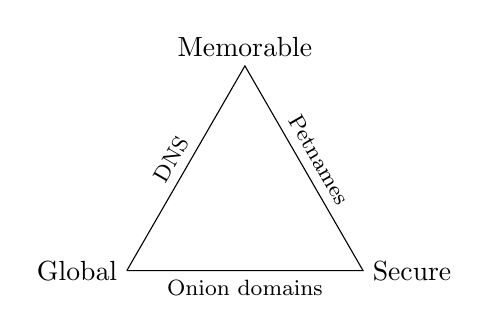
\begin{tikzpicture}

\draw (0.0,0.0) node[anchor=east] {Global}
        -- node [midway, below, sloped] {{\footnotesize Onion domains}}
      (3.0,0.0) node[anchor=west] {Secure}
        -- node [midway, above, sloped] {{\footnotesize Petnames}}
      (1.5,2.6) node[anchor=south] {Memorable}
        -- node [midway, above, sloped] {{\footnotesize DNS}}
      (0.0,0.0);

\end{tikzpicture}
\caption{``Zooko's triangle,'' a conjecture that posits that any naming scheme
can only satisfy two properties out of secure, memorable, and global.}
\label{fig:naming-triangle}
\end{figure}
